% ------------------------------------------------------------------------------
% TYPO3 CMS 8.6 - What's New - Chapter "Interface Utilisateur Backend" (French Version)
%
% @author	Michael Schams <schams.net>
% @license	Creative Commons BY-NC-SA 3.0
% @link		http://typo3.org/download/release-notes/whats-new/
% @language	French
% ------------------------------------------------------------------------------
% LTXE-CHAPTER-UID:		07b25346-95b1df21-a6ebe09a-49f53f41
% LTXE-CHAPTER-NAME:	Interface Utilisateur Backend
% ------------------------------------------------------------------------------

\section{Interface Utilisateur Backend}
\begin{frame}[fragile]
	\frametitle{Interface Utilisateur Backend}

	\begin{center}\huge{Chapitre 1~:}\end{center}
	\begin{center}\huge{\color{typo3darkgrey}\textbf{Interface Utilisateur Backend}}\end{center}

\end{frame}

% ------------------------------------------------------------------------------
% LTXE-SLIDE-START
% LTXE-SLIDE-UID:		4958421c-a927c714-a3b563bf-a3805973
% LTXE-SLIDE-ORIGIN:	4141a9cc-46da51df-9dd87a8b-9b15ac29 English
% LTXE-SLIDE-TITLE:		#12211: Scheduler Page Browser
% LTXE-SLIDE-REFERENCE:	!Feature: #12211 - Usability: Scheduler provide page browser to choose start page
% ------------------------------------------------------------------------------
\begin{frame}[fragile]
	\frametitle{Interface Utilisateur Backend}
	\framesubtitle{Navigateur de page du planificateur}

	Pour améliorer la facilité d'utilisation de la tâche planifiée
	\textbf{EXT:linkvalidator}, le navigateur de page est ajouté pour
	sélectionner la page de démarrage.

	\begin{figure}\vspace{-0.2cm}
		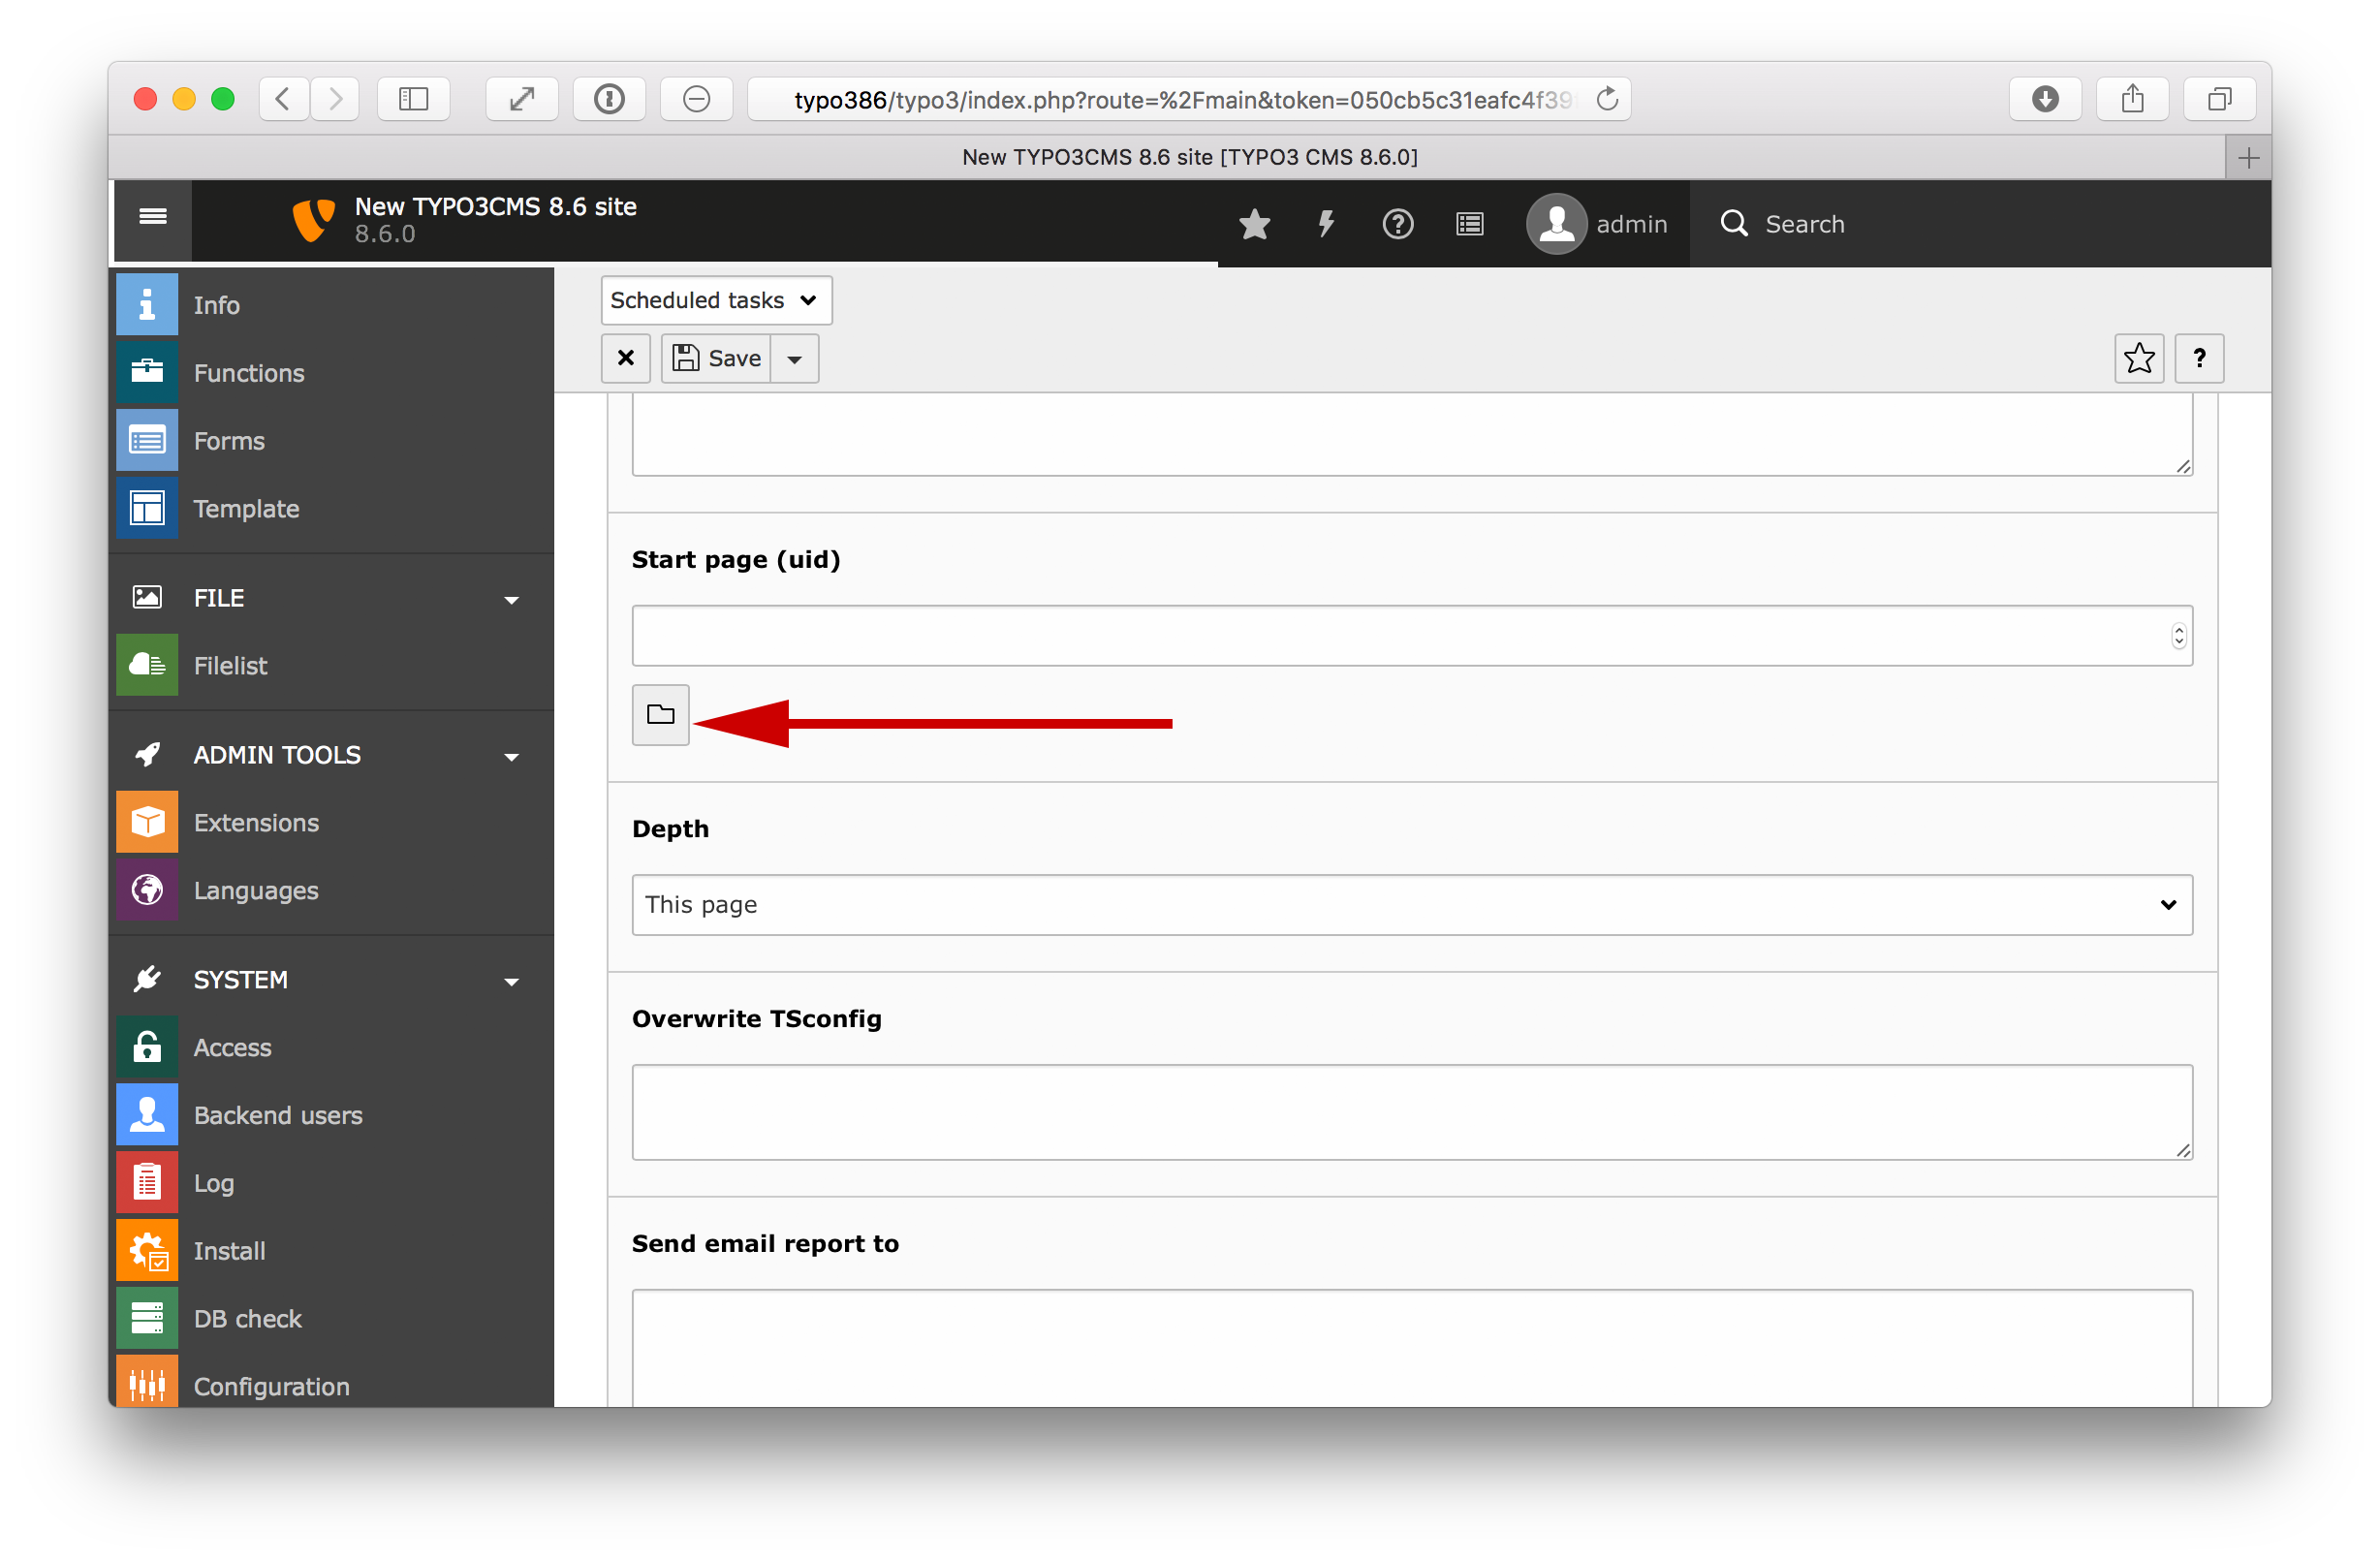
\includegraphics[width=0.67\linewidth]{BackendUserInterface/12211.png}
	\end{figure}

\end{frame}

% ------------------------------------------------------------------------------
% LTXE-SLIDE-START
% LTXE-SLIDE-UID:		1d8dbfef-945b787e-295cd5e6-0d748106
% LTXE-SLIDE-ORIGIN:	f924be39-75ae40d9-ba00f0a8-3a6de040 English
% LTXE-SLIDE-TITLE:		#45537: Manually executed tasks
% LTXE-SLIDE-REFERENCE:	!Feature: #45537 - Run manually executed tasks on next cron-run
% ------------------------------------------------------------------------------
\begin{frame}[fragile]
	\frametitle{Interface Utilisateur Backend}
	\framesubtitle{Planifier pour une exécution immédiate}

	\begin{columns}[T]
		\begin{column}{0.35\textwidth}
			Une icône d'action pour marquer une tâche à exécuter par la prochaine passe du
			planificateur est ajouté. Le bouton «~Exécuter les tâches sélectionnées lors de
			la prochaine exécution~» est aussi ajouté pour la même opération sur les tâches
			sélectionnées.
		\end{column}

		\begin{column}{0.65\textwidth}
			\begin{figure}\vspace{-0.6cm}
				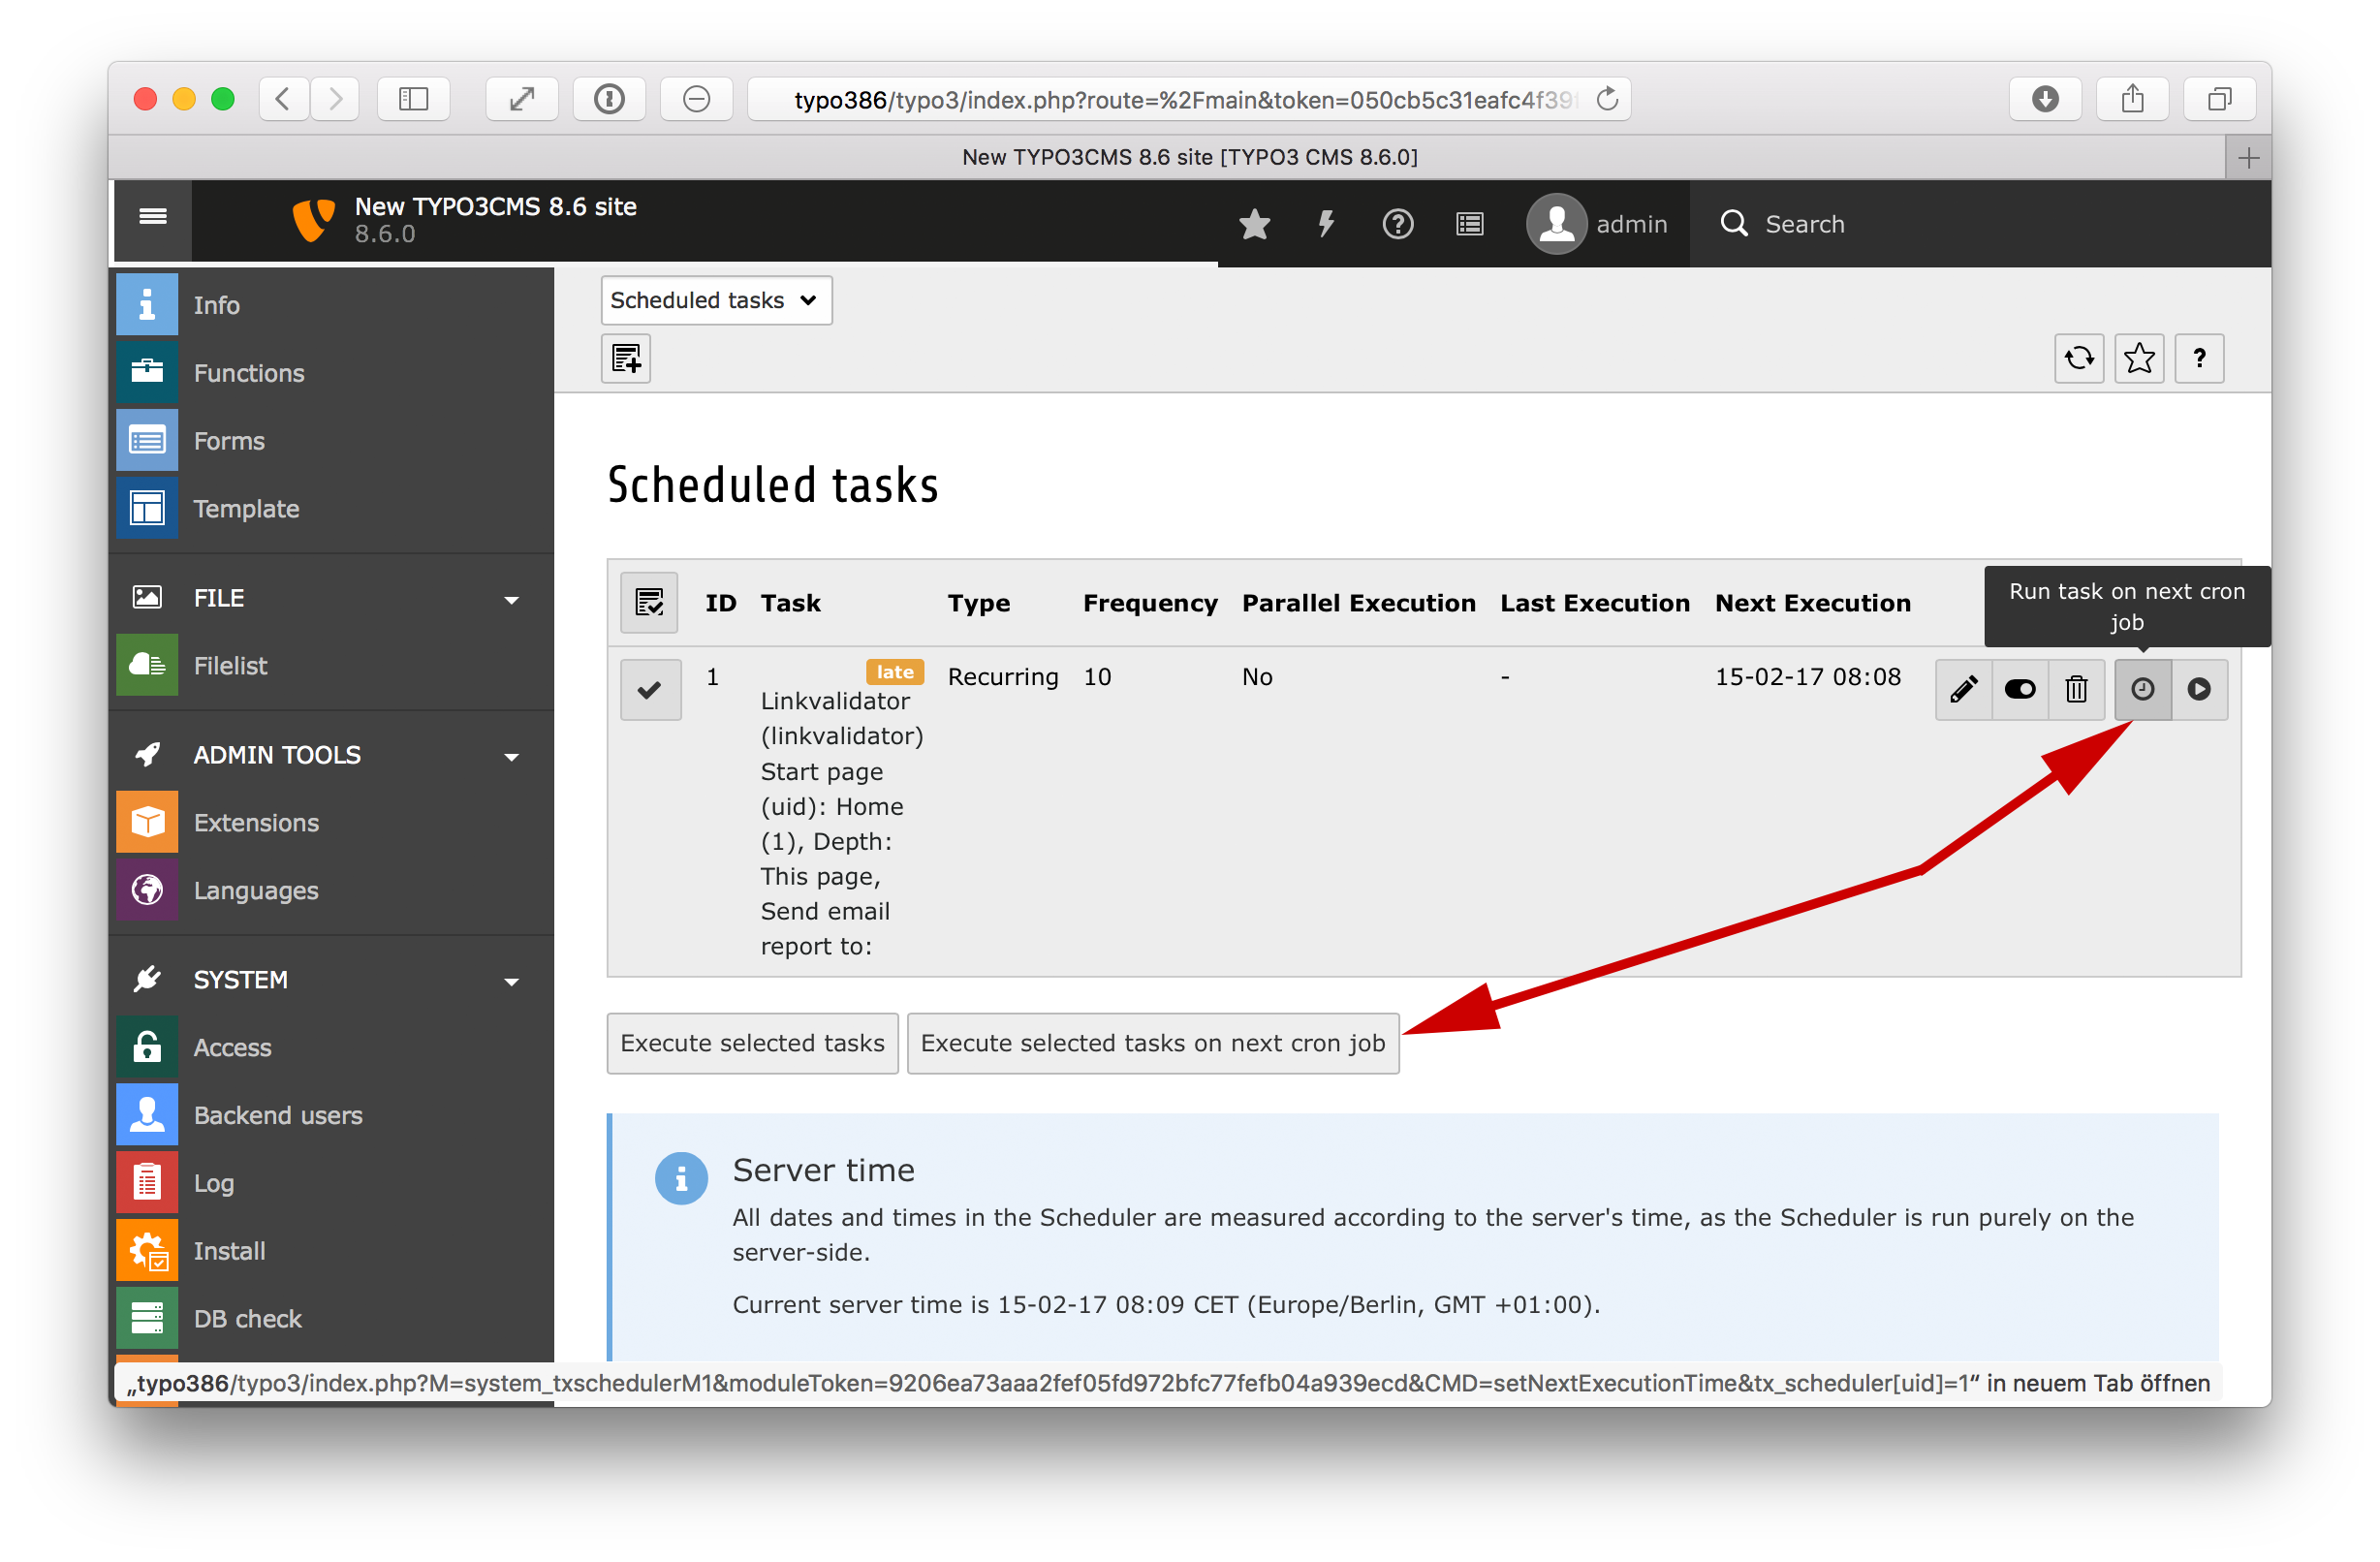
\includegraphics[width=0.99\linewidth]{BackendUserInterface/45537.png}
			\end{figure}
		\end{column}
	\end{columns}

\end{frame}

% ------------------------------------------------------------------------------
% LTXE-SLIDE-START
% LTXE-SLIDE-UID:		8564873b-654200d6-3990e0b5-a41a1f6c
% LTXE-SLIDE-ORIGIN:	b6d6054e-21291d35-479a0095-a6e82a4f English
% LTXE-SLIDE-TITLE:		#47135: Paste Icon and Modal
% LTXE-SLIDE-REFERENCE:	!Feature: #51291 - Synchronized field values in localized records
% ------------------------------------------------------------------------------
\begin{frame}[fragile]
	\frametitle{Interface Utilisateur Backend}
	\framesubtitle{Icône coller et confirmation}

	Dès que le presse papier normal contient un élément, une icône pour coller devient
	disponible dans le module page. Lorsque l'utilisateur clique dessus, une fenêtre
	apparaît à l'utilisateur pour confirmer l'action.

	\begin{figure}\vspace{-0.2cm}
		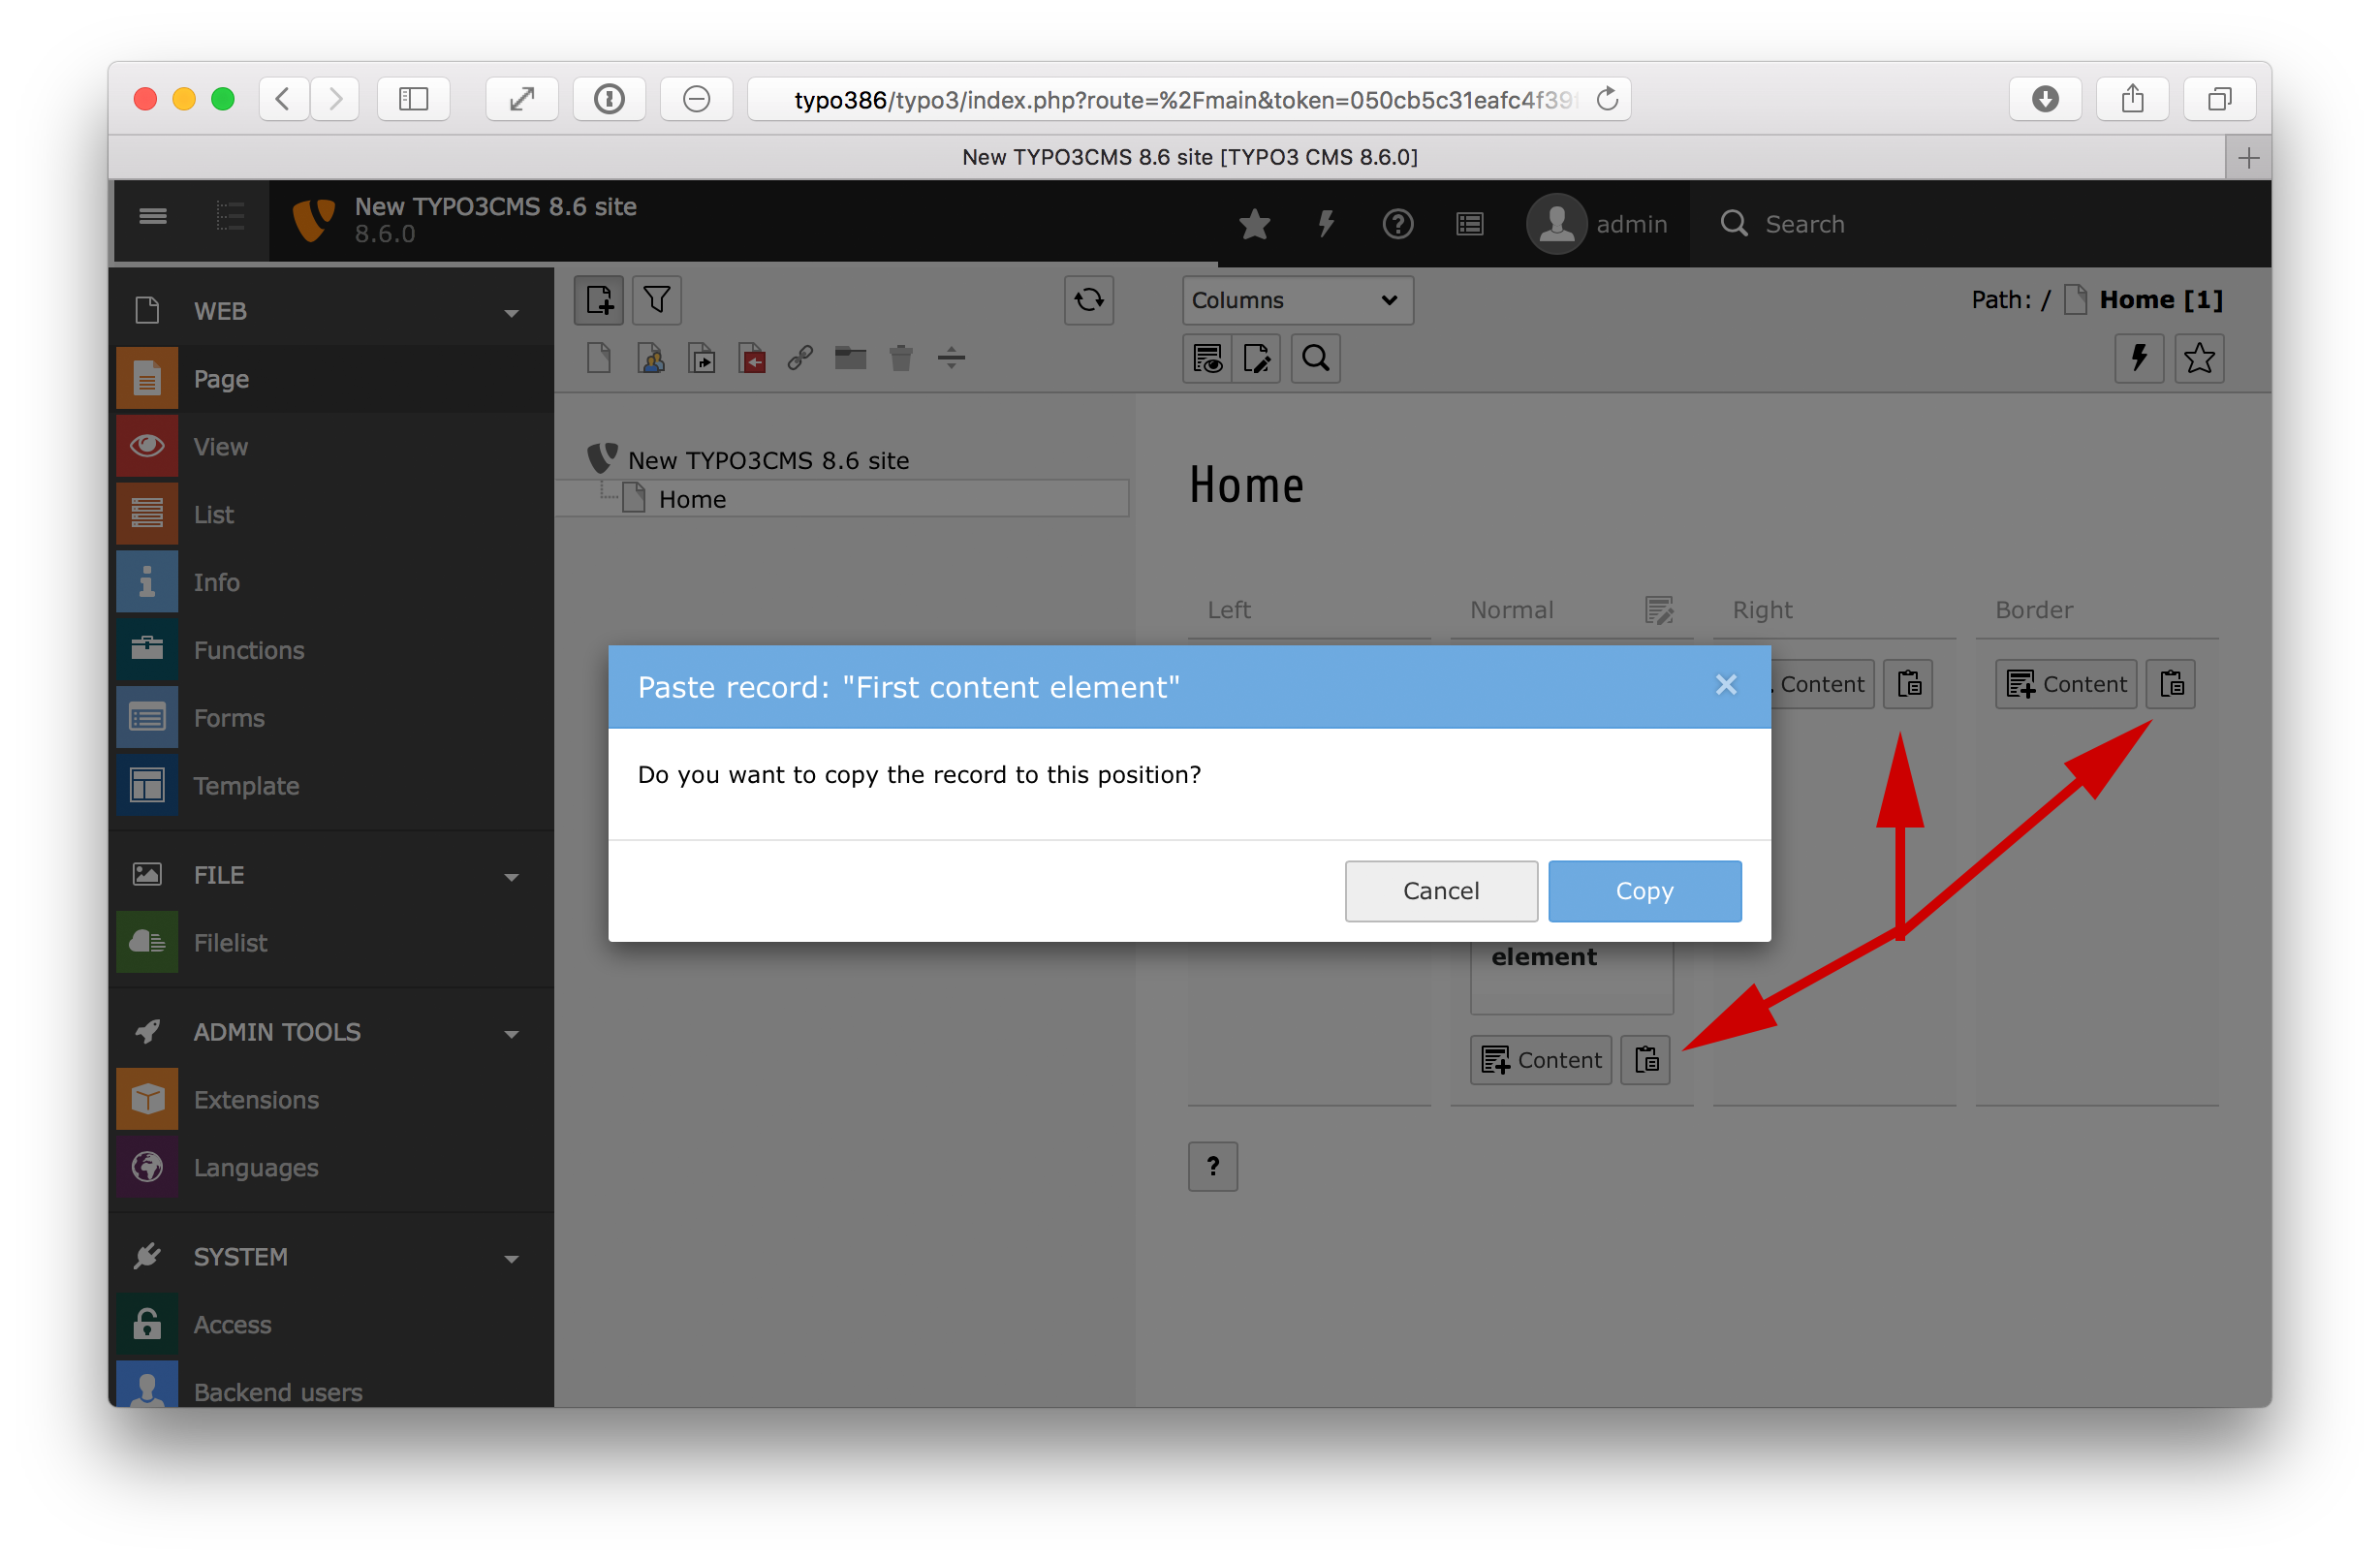
\includegraphics[width=0.63\linewidth]{BackendUserInterface/47135.png}
	\end{figure}

\end{frame}

% ------------------------------------------------------------------------------
% LTXE-SLIDE-START
% LTXE-SLIDE-UID:		ddeb4872-06f41f4b-56e0a0d9-79e9bba9
% LTXE-SLIDE-ORIGIN:	b31e455f-fce042ed-e3670436-9e72983c English
% LTXE-SLIDE-TITLE:		#67243: Folding of Scheduler Task Groups
% LTXE-SLIDE-REFERENCE:	!Feature: #67243 - Implement folding of scheduler task groups
% ------------------------------------------------------------------------------
\begin{frame}[fragile]
	\frametitle{Interface Utilisateur Backend}
	\framesubtitle{Replier les groupes de tâches}

	Lorsque les groupes de tâches sont utilisés, les tâches sont affichées groupées
	dans la liste. Cliquer la ligne avec le nom du groupe masque ou affiche les
	tâches du groupe.

	\begin{figure}\vspace{-0.3cm}
		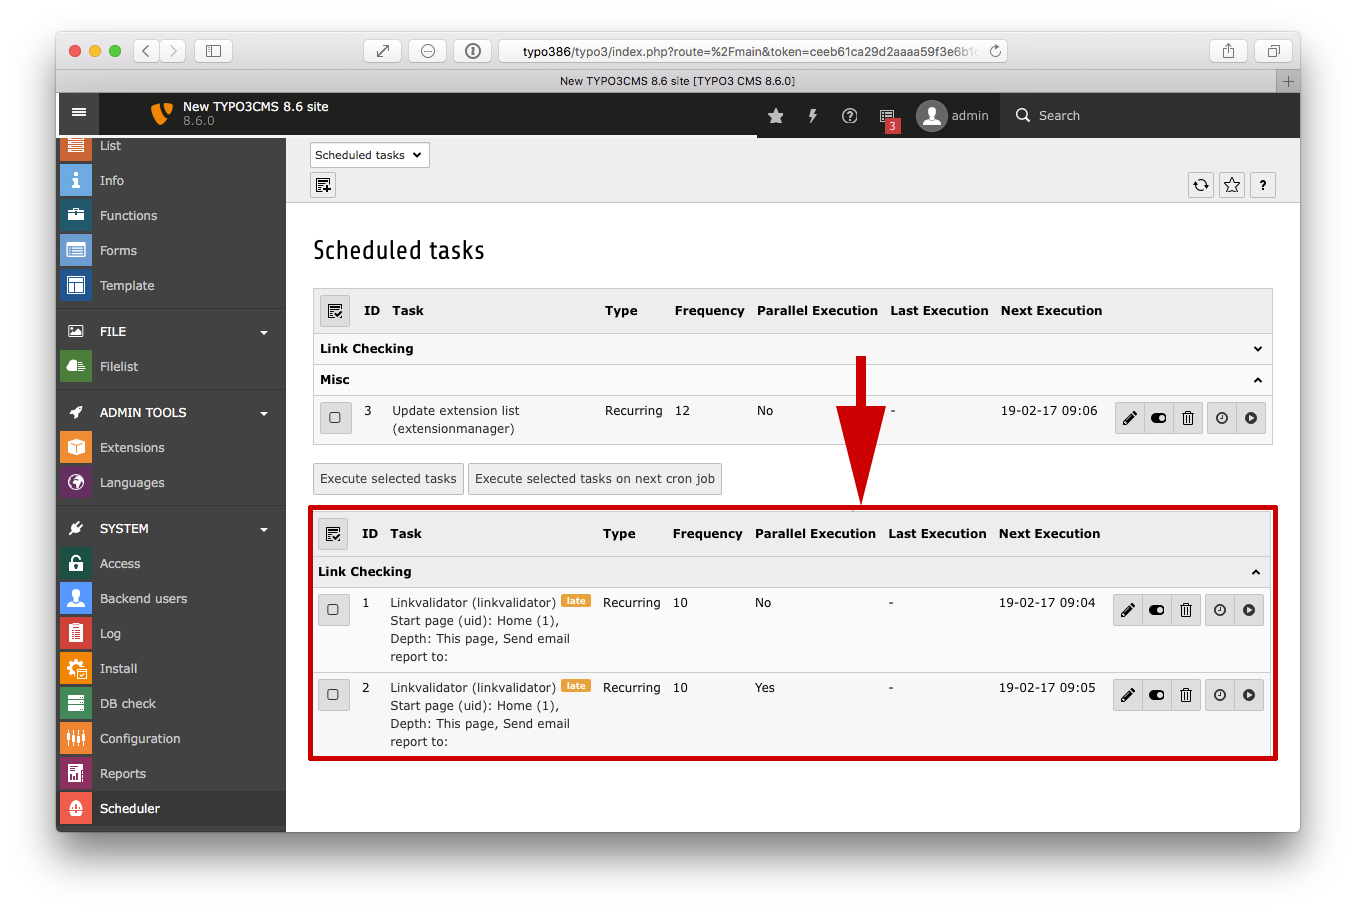
\includegraphics[width=0.60\linewidth]{BackendUserInterface/67243.png}
	\end{figure}

\end{frame}

% ------------------------------------------------------------------------------
% LTXE-SLIDE-START
% LTXE-SLIDE-UID:		bbe60eb4-89c321b8-1960b8c9-0e510be4
% LTXE-SLIDE-ORIGIN:	14fe5a0b-2a22a6ce-325b5de1-ef26ce50 English
% LTXE-SLIDE-TITLE:		#69572: Page Module Notice
% LTXE-SLIDE-REFERENCE:	!Feature: #69572 - Page module Notice "Content is also shown on:"
% ------------------------------------------------------------------------------
\begin{frame}[fragile]
	\frametitle{Interface Utilisateur Backend}
	\framesubtitle{Note du module page «~Contenu aussi affiché sur~»}

	\begin{columns}[T]
		\begin{column}{.3\textwidth}
			Lorsque du contenu de page est hérité depuis une page différente par «~Afficher
			le contenu depuis la page~», une note est affichée sur la page d'où provient le
			contenu.
		\end{column}

		\begin{column}{.7\textwidth}
			\begin{figure}\vspace*{-0.6cm}
				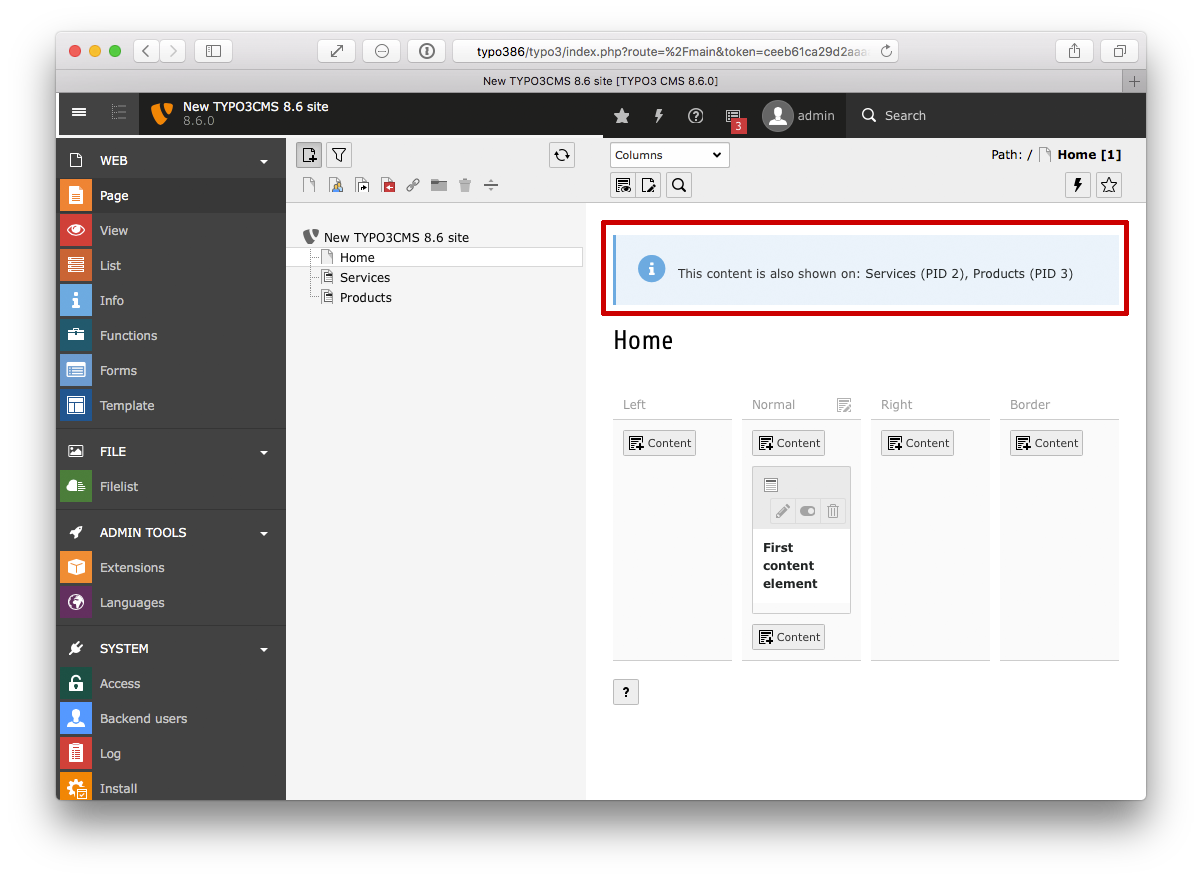
\includegraphics[width=\linewidth]{BackendUserInterface/69572.png}
			\end{figure}
		\end{column}
	\end{columns}

\end{frame}

% ------------------------------------------------------------------------------
% LTXE-SLIDE-START
% LTXE-SLIDE-UID:		40636e41-c584153e-28056322-4dc7cd8d
% LTXE-SLIDE-ORIGIN:	23a4baef-462e7d0c-c8cd4cfc-9dac1f99 English
% LTXE-SLIDE-TITLE:		#75880: Image Manipulation - Multiple Cropping Variants
% LTXE-SLIDE-REFERENCE:	!Feature: #75880 - Implement multiple cropping variants in image manipulation tool
% ------------------------------------------------------------------------------
\begin{frame}[fragile]
	\frametitle{Interface Utilisateur Backend}
	\framesubtitle{Manipulation d'images - Variantes de recadrage multiples}

	L'outil de manipulation d'image gère plusieurs variantes de cadrage (si configurées).
	Les utilisateurs peuvent aussi sélectionner une zone d'intérêt, qui soit toujours dans
	le cadre et marque la zone de l'image transportant son sens. Pour fournir aux éditeurs
	des indices à propos des zones de % -- beware of text flow here, it continues in the column

	\begin{columns}[T]
		\begin{column}{.35\textwidth}
			l'image utilisées par d'autres éléments comme les en-têtes, lors de la sélection
			d'une zone de cadrage, il est possible de définir de multiples zones de couverture.
		\end{column}

		\begin{column}{.65\textwidth}
			\begin{figure}\vspace*{-0.6cm}
				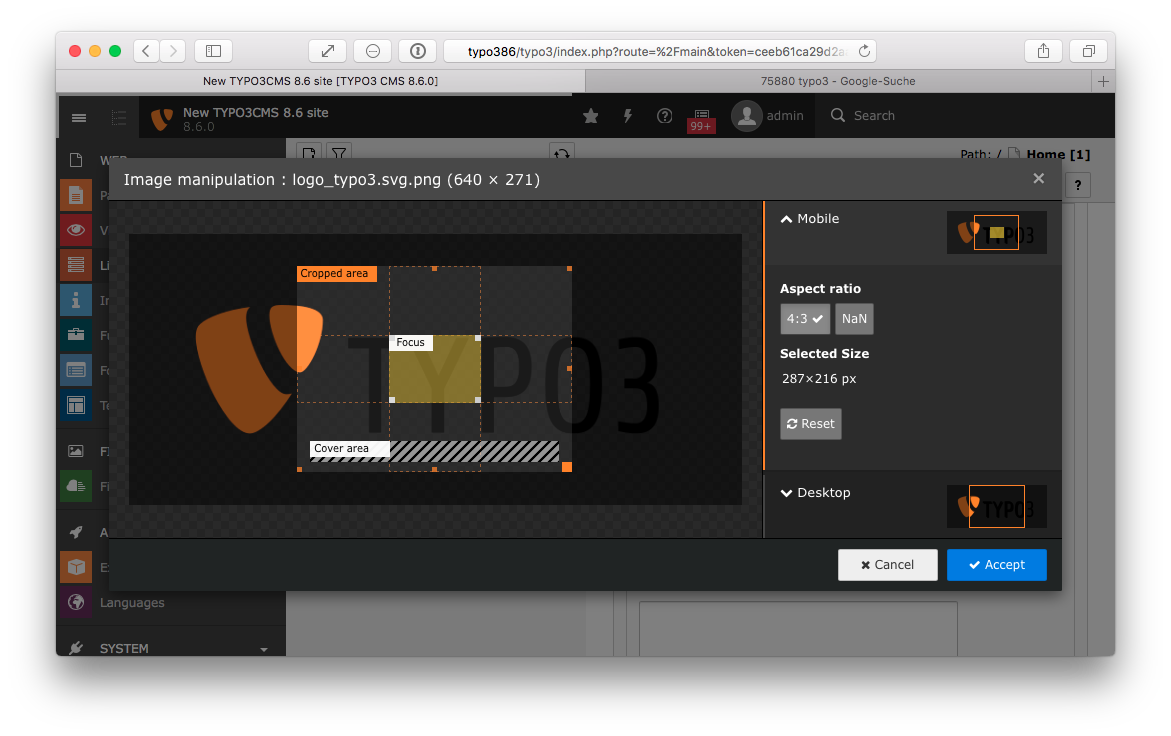
\includegraphics[width=0.99\linewidth]{BackendUserInterface/75880.png}
			\end{figure}
		\end{column}
	\end{columns}

\end{frame}

% ------------------------------------------------------------------------------
% LTXE-SLIDE-START
% LTXE-SLIDE-UID:		5cb287e7-db2830f2-dbac2f7b-ea3d1215
% LTXE-SLIDE-ORIGIN:	8f2f695d-f5c6a8bf-5700cf34-d6389ce8 English
% LTXE-SLIDE-TITLE:		#79235: Delete Similar Errors (sys_log)
% LTXE-SLIDE-REFERENCE:	!Feature: #79235 - Add button to delete similar errors from sys_log
% ------------------------------------------------------------------------------
\begin{frame}[fragile]
	\frametitle{Interface Utilisateur Backend}
	\framesubtitle{Supprimer les erreurs similaires du \texttt{sys\_log}}

	Le module journal de TYPO3 affiche un bouton pour supprimer plusieurs erreurs à la fois
	en se basant sur le champ \texttt{details} de la table \texttt{sys\_log}. Pratique
	lorsque l'on vient de corriger une erreur récurrente.

	\begin{figure}\vspace{-0.2cm}
		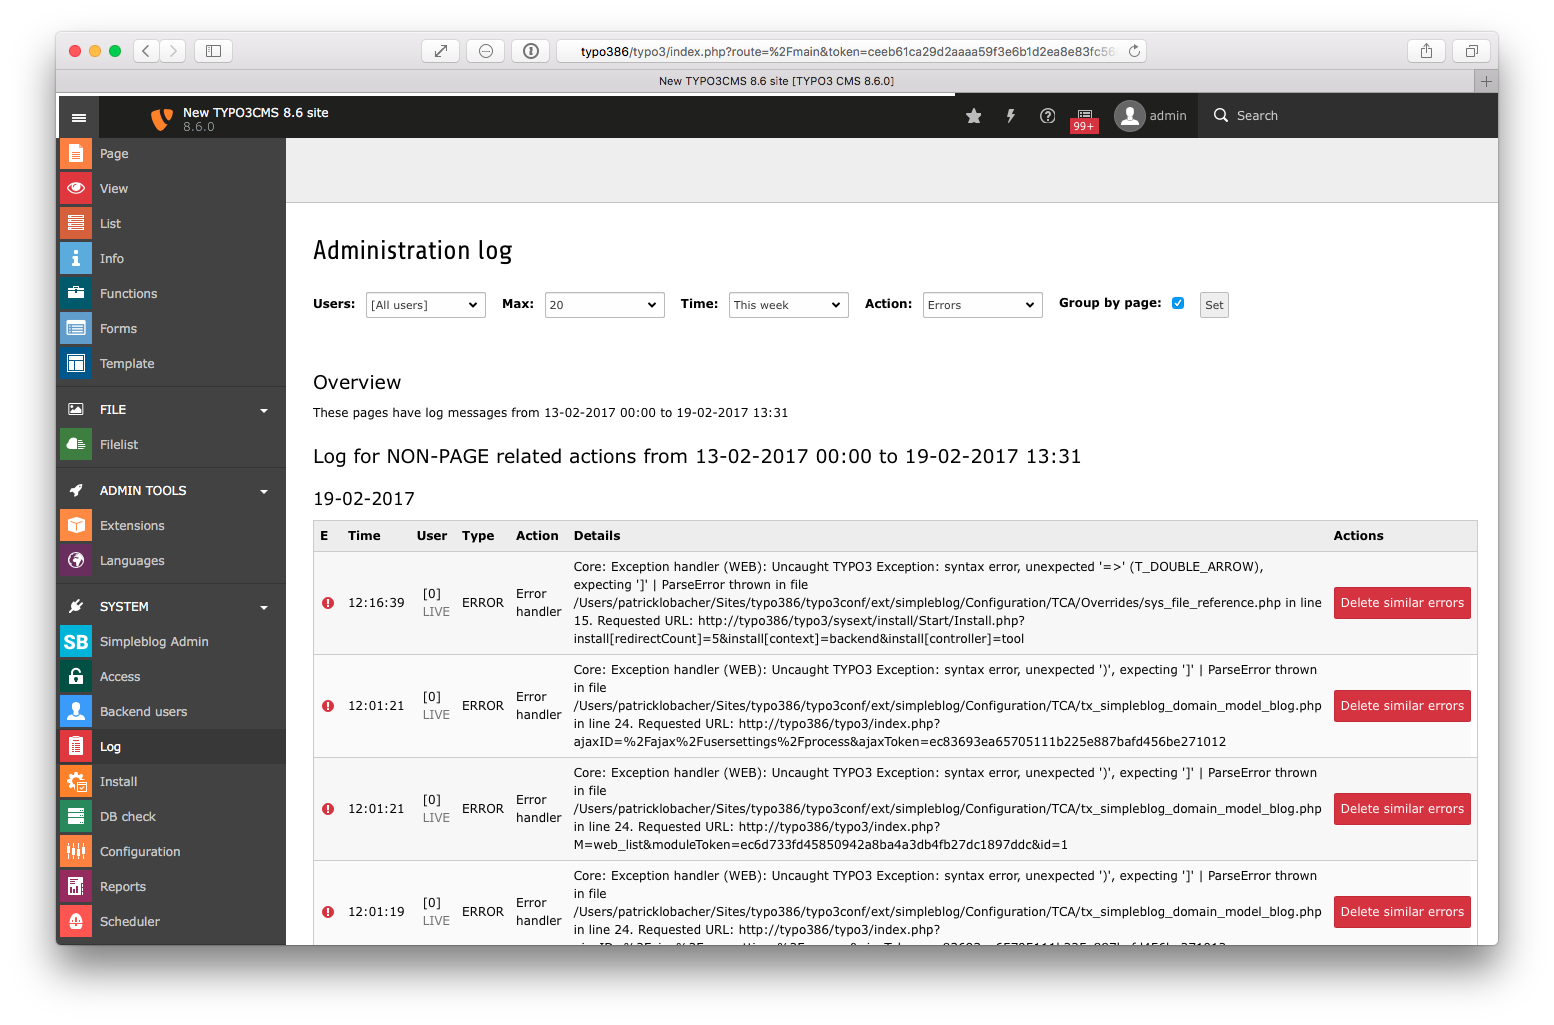
\includegraphics[width=0.60\linewidth]{BackendUserInterface/79235.png}
	\end{figure}

\end{frame}

% ------------------------------------------------------------------------------
% LTXE-SLIDE-START
% LTXE-SLIDE-UID:		ddd561ac-fa794b98-d839b2f0-66bc9940
% LTXE-SLIDE-ORIGIN:	fc878ad9-7b163d51-e579b8b3-9cbe41d9 English
% LTXE-SLIDE-TITLE:		#79467: Form settings button
% LTXE-SLIDE-REFERENCE:	!Feature: #79467 - EXT:form - add form settings button to module header
% ------------------------------------------------------------------------------
\begin{frame}[fragile]
	\frametitle{Interface Utilisateur Backend}
	\framesubtitle{\texttt{EXT:form}~: bouton d'options dans l'en-tête}

	Un nouveau bouton est ajouté à l'en-tête de module de l'éditeur de formulaire.
	Cliquer sur ce bouton affiche les options de formulaire dans la colonne de propriétés.

	\begin{figure}\vspace{-0.2cm}
		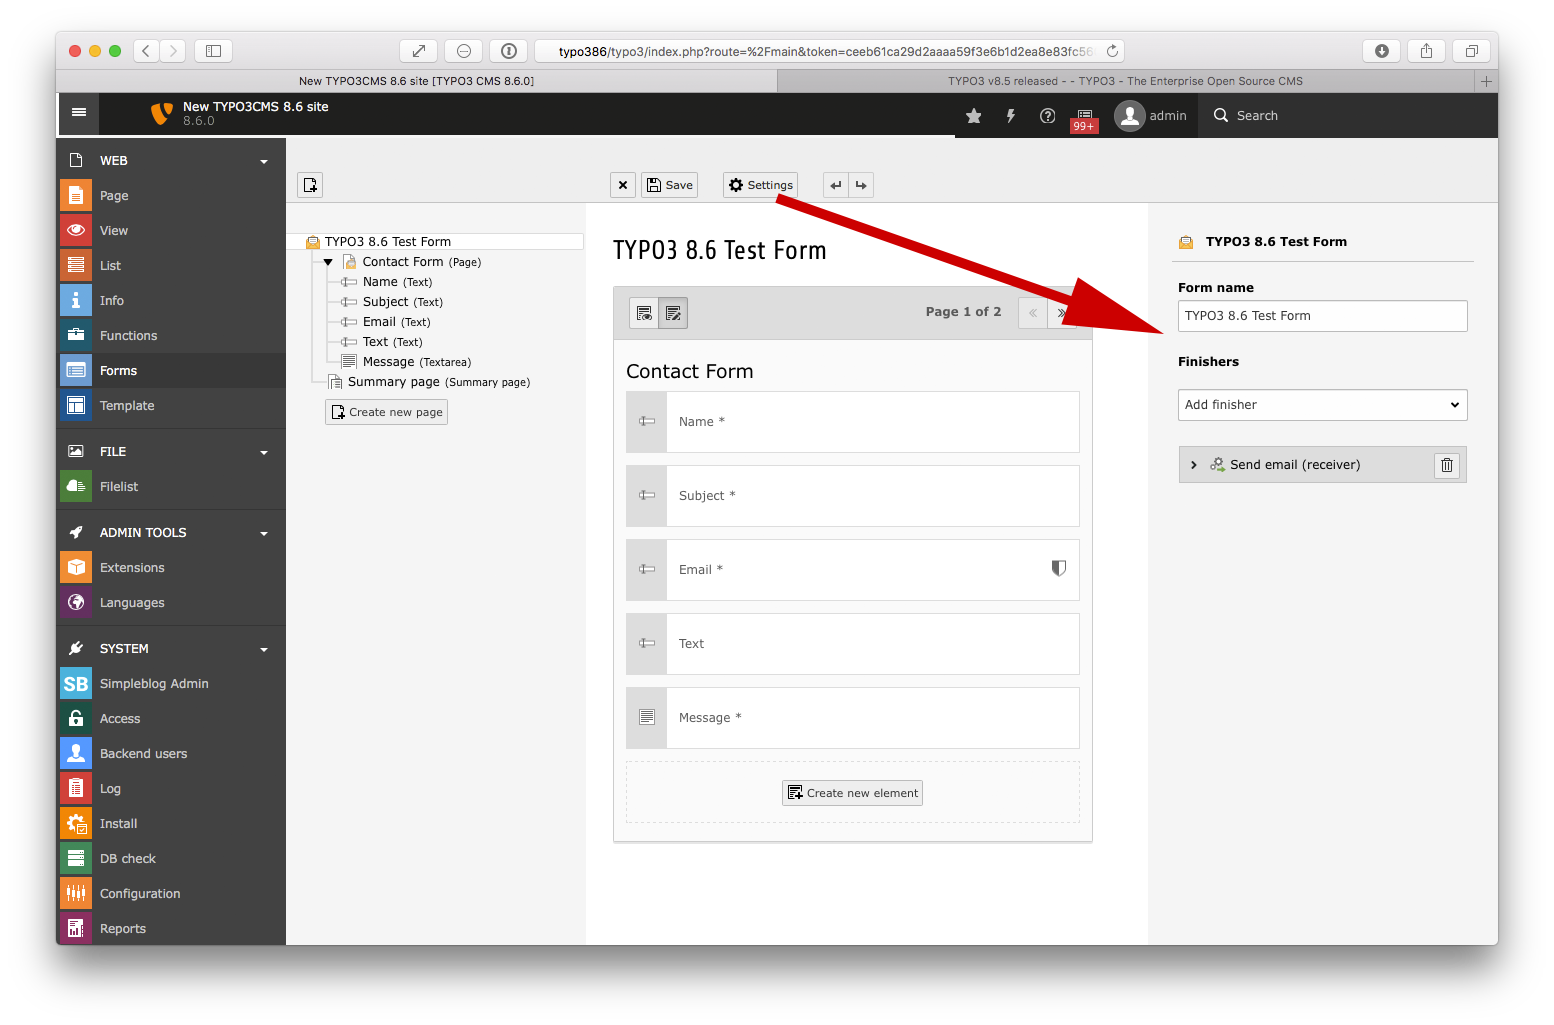
\includegraphics[width=0.675\linewidth]{BackendUserInterface/79467.png}
	\end{figure}

\end{frame}

% ------------------------------------------------------------------------------
% LTXE-SLIDE-START
% LTXE-SLIDE-UID:		dc1d73fd-10c5ad2a-2e593749-96a5ae81
% LTXE-SLIDE-ORIGIN:	e1759d2e-8cc138ca-40ce6a34-65354b0e English
% LTXE-SLIDE-TITLE:		#79531: EXT:form - Add multiselect inspector editor
% LTXE-SLIDE-REFERENCE:	!Feature: #79531 - EXT:form - Add multiselect inspector editor
% ------------------------------------------------------------------------------
\begin{frame}[fragile]
	\frametitle{Interface Utilisateur Backend}
	\framesubtitle{{EXT:form}~: ajout de l'éditeur pour multiselect}

	\begin{columns}[T]
		\begin{column}{0.4\textwidth}
			Un nouvel éditeur de propriétés, c-à-d un nouveau type de l'éditeur de formulaire,
			est ajouté. Si appliqué, les champs de sélection multiple deviennent disponibles.
			Un champ de sélection multiple permet la sélection de propriétés multiples pour un
			champ et les enregistres dans la propriété indiquée.
		\end{column}

		\begin{column}{0.6\textwidth}
			\begin{figure}\vspace*{-0.6cm}
				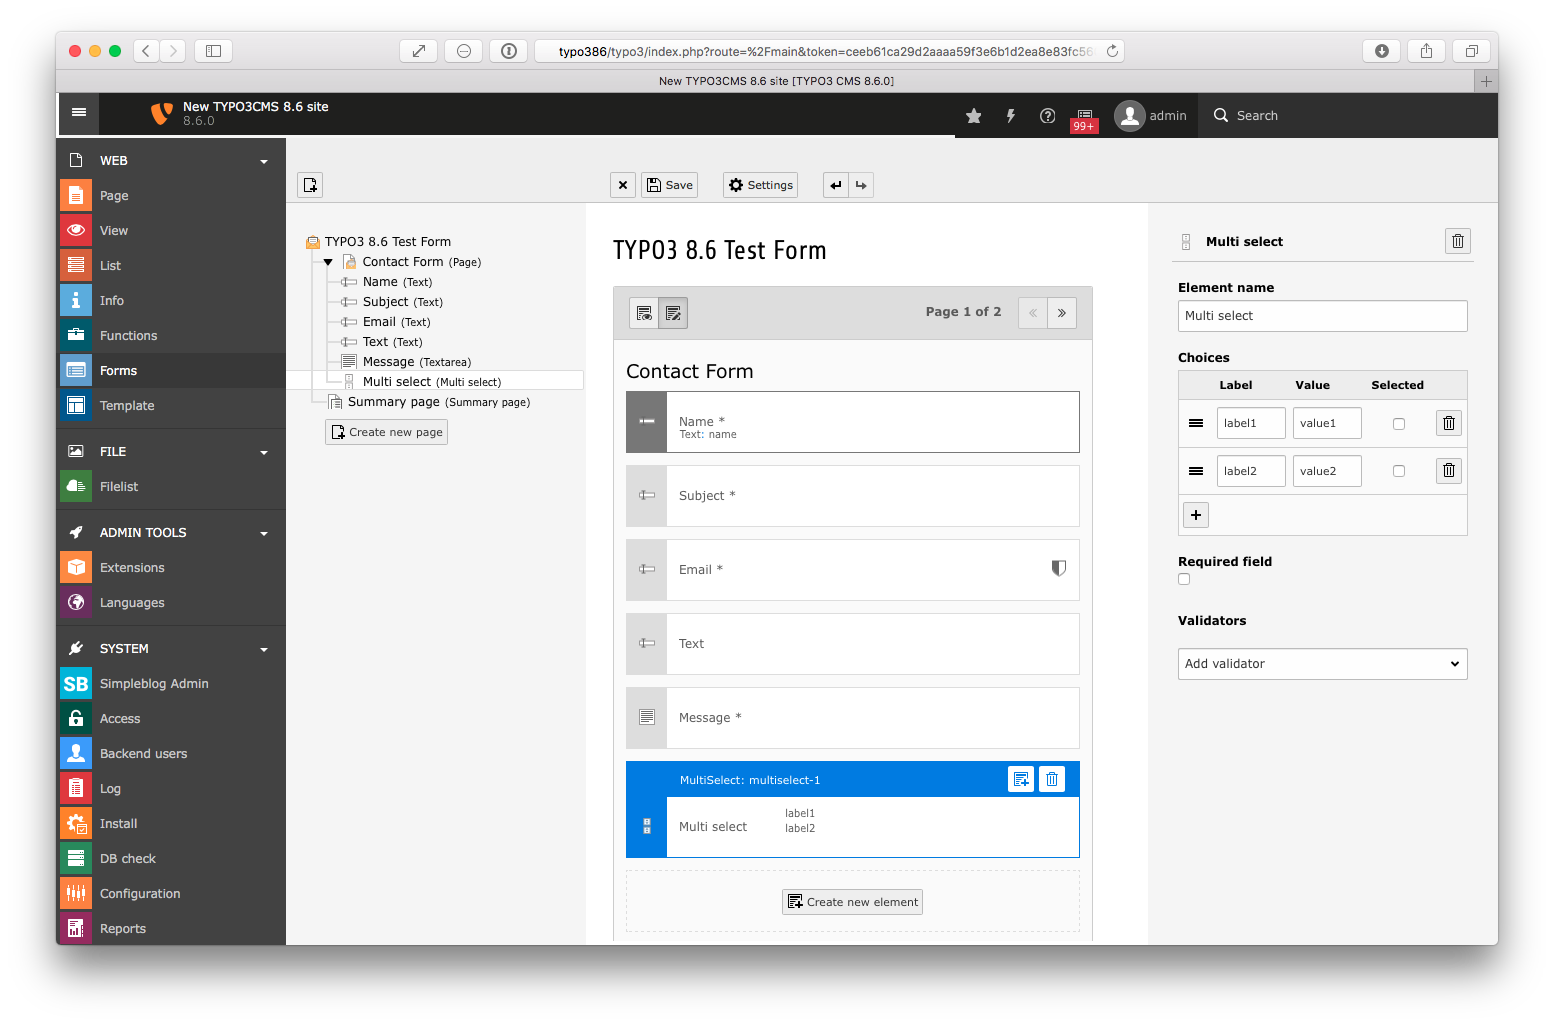
\includegraphics[width=0.99\linewidth]{BackendUserInterface/79531.png}
			\end{figure}
		\end{column}
	\end{columns}

\end{frame}

% ------------------------------------------------------------------------------
% LTXE-SLIDE-START
% LTXE-SLIDE-UID:		7de6bdc6-e7644f7a-4106d9b0-bce7427b
% LTXE-SLIDE-ORIGIN:	f6756002-b9aac45f-9460b472-1da819b5 English
% LTXE-SLIDE-TITLE:		#79521: Show list of failed input elements in FormEngine
% LTXE-SLIDE-REFERENCE:	!Feature: #79521 - Show list of failed input elements in FormEngine
% ------------------------------------------------------------------------------
\begin{frame}[fragile]
	\frametitle{Interface Utilisateur Backend}
	\framesubtitle{Liste des erreurs de validation FormEngine}

	\begin{columns}[T]
		\begin{column}{.35\textwidth}
			Lorsque la validation des champs de FormEngine échoue, un bouton est ajouté dans la
			barre des boutons de l'en-tête de module. Le clic sur ce bouton affiche une liste des
			champs d'entrée dont la validation a échoué. Le clic sur un champ l'active dans le
			formulaire.
		\end{column}

		\begin{column}{.65\textwidth}
			\begin{figure}\vspace*{-0.6cm}
				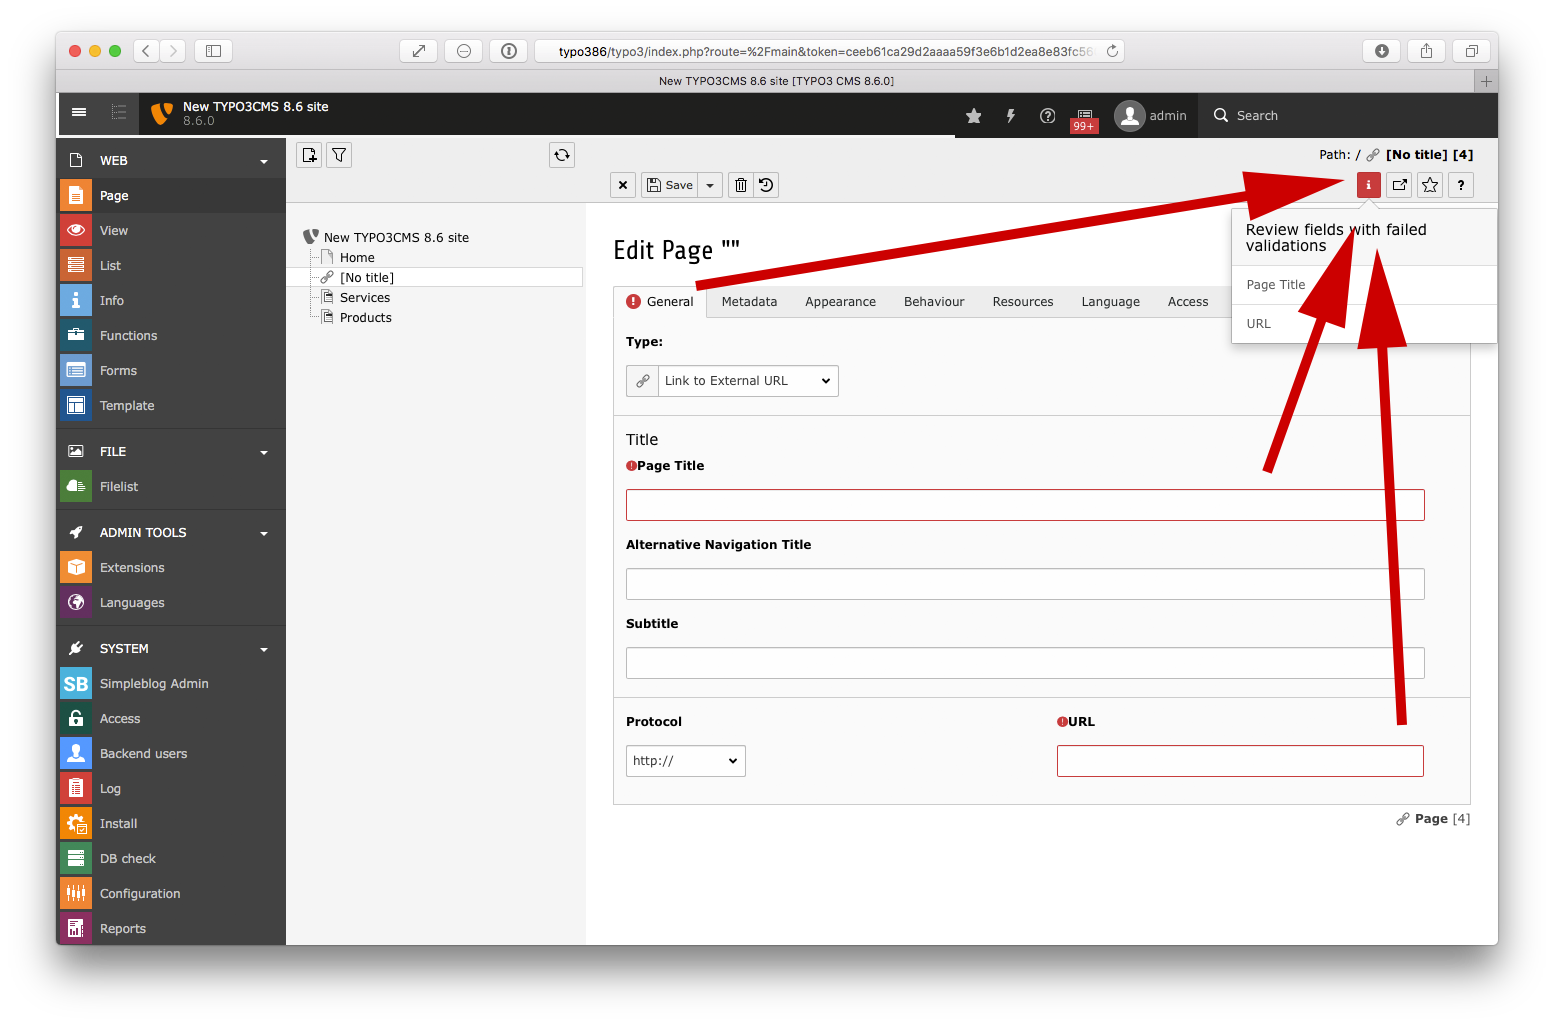
\includegraphics[width=0.99\linewidth]{BackendUserInterface/79521.png}
			\end{figure}
		\end{column}
	\end{columns}

\end{frame}

% ------------------------------------------------------------------------------
% LTXE-SLIDE-START
% LTXE-SLIDE-UID:		b7cad5e0-c59b7c32-ba11fa47-697aad23
% LTXE-SLIDE-ORIGIN:	749a055b-02003192-92f2631e-39abcc95 English
% LTXE-SLIDE-TITLE:		#79622: Dedicated content elements for menus
% LTXE-SLIDE-REFERENCE:	!Breaking: #79622 - Dedicated content elements for menus
% ------------------------------------------------------------------------------
\begin{frame}[fragile]
	\frametitle{Interface Utilisateur Backend}
	\framesubtitle{Éléments de contenu dédiés pour les menus}

	Pour faciliter la maintenance, les éléments de contenu de menu actuels ont été
	répartis dans des éléments dédiés.

	\begin{figure}\vspace{-0.2cm}
		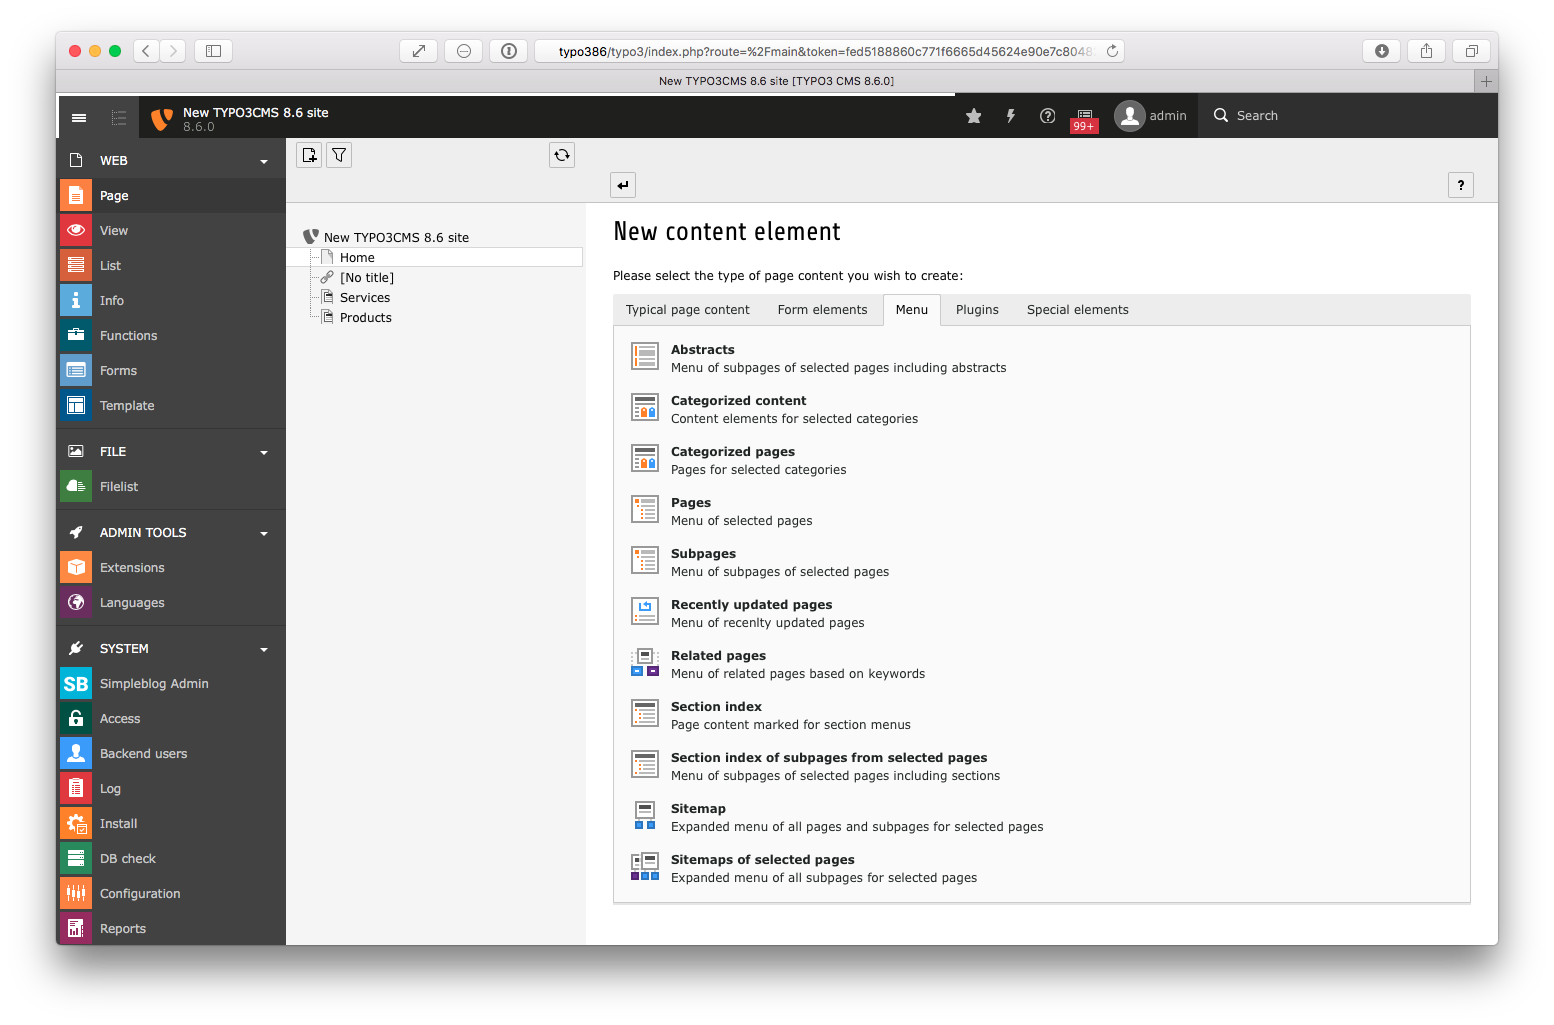
\includegraphics[width=0.68\linewidth]{BackendUserInterface/79622.png}
	\end{figure}

\end{frame}

% ------------------------------------------------------------------------------
